% !TEX root = ../main.tex

\chapter{基于符号回归的系统动态特征学习与应用}
\label{chap:symbolic-regression}

\section{引言}
\label{sec:sr-intro}
%axle:轮轴(车轴),bearing:轴承
% 铁路运输的重要性,高速列车的安全问题和维修成本问题。
铁路运输具有规模大、经济、节能等优势使其在人类社会中扮演着重要角色。以中国铁路运输为例,支持中国25\%的运输量,能源消耗仅占所有运输方式总消耗的6\%\cite{2015年交通运输行业发展统计公报}。在可持续发展的需求下,铁路运输将会在人类社会中扮演更重要的角色,比如截止 2016 年底,中国“四纵四横”高速 铁路基本成型,即将迎来“八纵八横”的新时代\cite{中长期铁路网规划}。然而,高速列车因其具有载客量大、运输速度快、行车密度 高等特点存在不容忽视的安全隐患,一旦发生事故将可能造成灾难性后果。 由于缺乏有效的故障诊断技术和策略,铁道部门只能采用不计成本保安全的劳动密集型计划维修体制,现有检测仪器只能通过局部物理信号进行阈值分析,结合专家经验与感觉器官进行故障诊断。维修效率低、费时费力、难以甚至不可能发现潜在安全隐患,由此产生的高维修支出难以支持中国高铁的可持续发展。

% PHM 技术在实际应用中的局限。
随着科技的进步和工业系统维修需求的高涨,融合传感器技术、领域知识和数据科学的故障预测和健康管理(PHM)技术逐渐被广泛关注、研究和应用\cite{lee2014prognostics,彭宇2010故障预测与健康管理技术综述}。然而 PHM 技术在机车系统中的应用仍存在诸多挑战:(1)现代机车已演变成高度复杂的工程机械,其正常运行需要依赖多个物理学科的统一,涉及力学、热力学、机电、电子、计算机和控制工程。(2)不同的运输目标和环境要求机车模型必须具备多样化特性。实际上机车服务年限已长达30年,系统化的 PHM 方案必须能应对多种机车组的不同需求。(3)制造业的全球化进程和复杂的设备所有权关系使建立具有全面领域知识的知识库面临巨大困难,甚至不可行。
%(1)现代机车已演变成高度复杂的工程机械,其正常运行需要依赖多个物理学科的统一,涉及力学( Mechanics)、热力学(Thermodynamics)、机电(Electromechanics)、电子(Electronics)、计算机(Computers)和控制工程(Control engineering)。

本文认为兼顾知识发现和故障预测的数据驱动方法是为国家铁路系统列车组提供完备PHM解决方案的唯一出路\cite{tsui2015prognostics, esling2012time, gaber2005mining, si2011remaining}。而对于数据驱动的PHM技术还需面对的额外挑战是:传感器数据的传输受限于可用传输带宽,并且复杂的数据采集和传输环境容易导致数据丢失或噪声引入的情况。因此数据驱动的PHM技术必须具备处理不确定因素和提取准确的有价值的信息的能力。

% 现有研究的不足并提出本章的研究点
现有的数据驱动故障预测方法主要以时间序列预测技术为基础,并且时间序列预测技术已受到广泛关注和验证,比如金融领域、工程领域和社会科学领域等\cite{brockwell2016introduction}。然而现有大多方法均以,比如ARIMA、VAR等,固定的模型结构为基础,很难反应系统在多种条件影响下的动态特性,无法揭示系统底层的物理机理。
%再者实践中发现当列车临近失效时ARIMA和VAR等传统时间序列预测模型无法工作。

综上所述,如何利用先进的数据驱动方法为高速列车组提供切合实际且完备的PHM解决方案仍然面临巨大挑战。本文在广泛而深入的调研以及实际项目考察的基础上提出基于符号回归的系统动态特征学习框架,并融合遗传算法和确定性优化算法训练模型,通过学习的系统方程了解系统的动态特征和底层物理机理。进一步,本文利用学习的系统动态方程构建时间序列预测模型形成完备的在线实时异常检测系统。

% 综上所述,如何利用先进的数据驱动方法为高速列车组提供切合实际且完备的 PHM 解决方案仍然面临巨大挑战。本文对先进的数据驱动的PHM技术框架进行深入研究并在此基础上为实际项目背景下的高速列车组设计和实现完备的故障诊断和故障预测框架。首先,本文以实际项目采集的温度数据为主要数据源,原因主要有以下两点:(1)实际项目考察中发现,温度传感器已经得到了更广泛的部署;(2)近年来已有重要的研究工作关注热轮轴温度的预测问题\cite{ma2016prediction,yi2015faults,amini2016wayside},在一定程度上说明了温度数据对系统性能的敏感性。进一步,本文以基于遗传算法的符号回归方法来学习系统动态方程,并基于此构建时间序列预测模型进而实现实时的故障诊断和故障预测。相比于传统时间序列预测方法,基于遗传算法的符号方法具有模型选择和参数学习能力、纯数据驱动、不受函数制约全方位搜索解空间以达到全局收敛等诸多优势,因此对物理系统底层动态特性具有很强的抽象学习能力,并且在实践中,即使列车临近失效模型仍能继续正常工作。

% % 研究结果。
% 本章设计的方案和框架部已署于实际项目的机车监控数据中心,支持故障诊断和故障预测任务,其有效性得到了实际项目的验证。此外,与典型的依赖领域知识从实验数据中抽取特征以支撑异常检测和故障预测的数据驱动的PHM框架不同,本文的架构直接利用传感器温度数据实现离线和在线的故障诊断和预测,由此证明了现代数据挖掘技术可以通过温度数据揭示轴承的动态性并可基于此执行精确的预测。

%We prove that modern data mining techniques are able to identify the internal dynamics of bearing through the temperature data and perform accurate prediction.

%In this work, we develop a hot-axle prediction and analysis framework. The framework is deployed in the locomotive monitoring data center to perform online fault prediction and diagnosis. It takes the multivariate sensor time series as input. The details of sensor data are listed in Table 1

%Different from existing data driven PHM studies, which typically use experimental data to extract patterns for anomaly detection/prediction under the guidance of domain knowledge, our framework performs online and off-line fault prediction by exploiting sensor data collected during regular operations. We prove that modern data mining techniques are able to identify the internal dynamics of bearing through the temperature data and perform accurate prediction

\section{数据采集和数据分析}

\subsection{数据采集}

实际工程项目中温度传感器已得到广泛部署,因此温度数据最为丰富。数据采集的设备和机车环境如图\ref{fig:sr-data-collect}所示。一辆机车有6个轮轴,每个轮轴配置8个传感器,这些传感器都统一配置为温度传感器。每个轮轴的8个传感器被部署于不同位置,其中2个分别放置于轮轴两端以感知环境温度,剩下的6个传感器均匀的分配到轮轴的2个轴承上。每个轴承有3个传感器,分别部署在轴承的左上方、上方和右上方。除了关键的轴承温度外,本文还采集了火车管道压力、停车制动压力、平衡油缸压力、火车管流和机车运行速度数据,具体的数据说明见表\ref{tab:sr-variables}。
\begin{figure}[H]
\centering
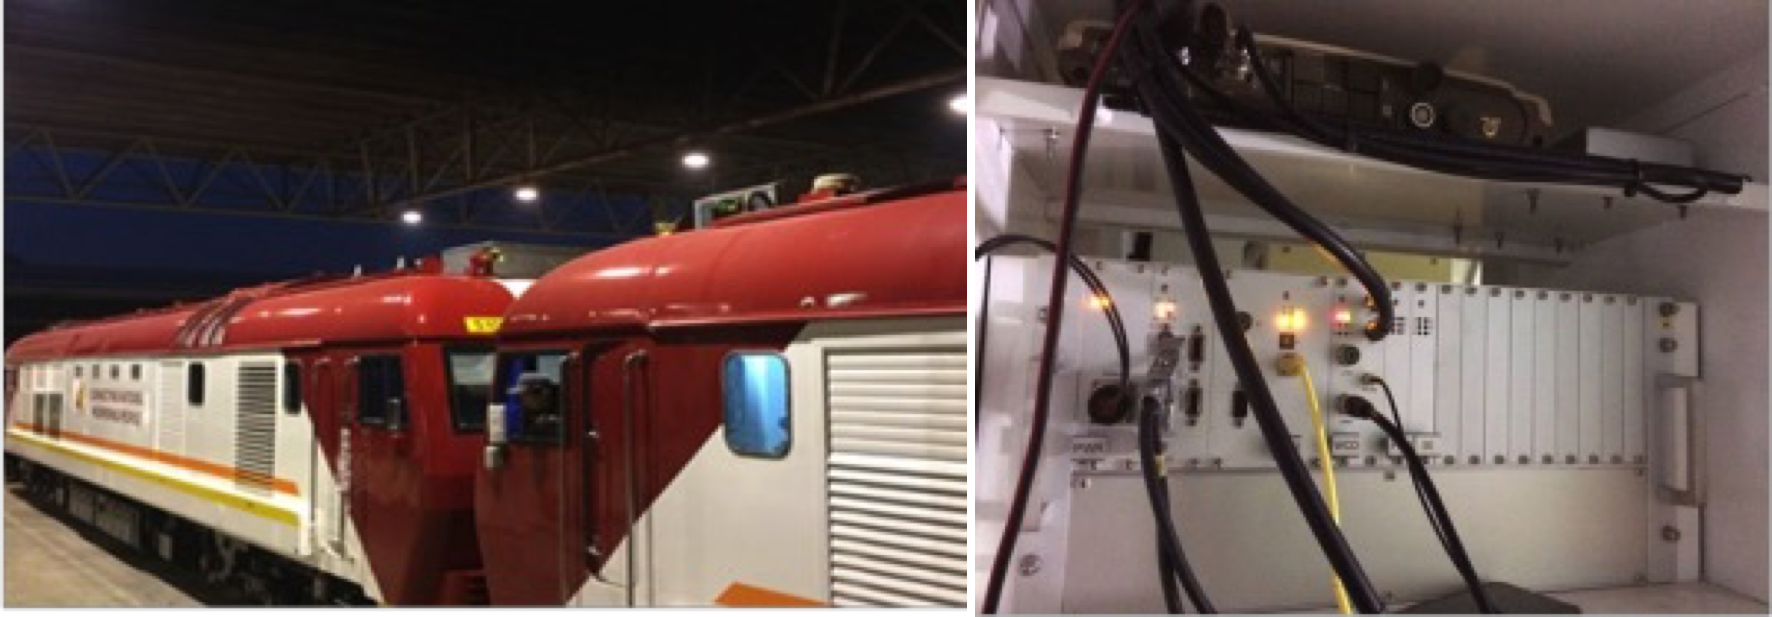
\includegraphics[scale=0.5]{figures/sr-data-collect.png}
\caption{机车和数据采集设备}
\label{fig:sr-data-collect}
\end{figure}
\begin{table}[htb]
  \centering
  \caption{高速列车走行部的多元时间序列数据}
  \label{tab:sr-variables}
    \begin{tabularx}{\linewidth}{XX}
      \toprule[1.5pt]
      {\heiti 变量名} & {\heiti 描述} \\\midrule[1pt]
      ZD\_LCG & 火车管道压力 \\
      ZD\_TFG & 停车制动压力 \\
      ZD\_JHG & 平衡油缸压力 \\
      ZD\_LLJ & 火车管流 \\
      ZD\_SPEED & 机车运行速度 \\
      ZD\_HW\_N\_1 & 轴承 N 左边的环境温度 \\
      ZD\_HW\_N\_2 & 轴承 N 右边的环境温度 \\
      ZD\_WD\_N\_Y & 轴承 N 在位置 Y 的温度 \\
      \bottomrule[1.5pt]
    \end{tabularx}
\end{table}

\subsection{数据分析}

(1)数据预处理

本文数据预处理主要由三部分组成。(1)数据集成:汇总不同维度的传感器数据并进行时间对标以保证数据的一致性。(2)数据清洗:本文首先基于少量先验知识去掉明显冗余的数据。针对传感器在数据采集过程中由于受到复杂环境的影响,存在数据丢失和噪音的情况,本文通过平滑处理方法消除干扰噪音(比如去除固定幅度和时间间隔的周期性波动噪音)。(3)重采样:符号回归模型存在一个隐含假设,即要求输入的时间序列数据必须为等时间间隔采的结果,而实际采集的数据由于受到缺失值和噪音的影响无法满足以上模型假设,对此本文采用适当的重采样技术对传感时间序列进行预处理以保证各采样点之间保持相等的时间间隔\cite{good2006resampling},通过多次实验验证发现高斯插值对数据处理的效果最好。
\begin{figure}[H]
\centering
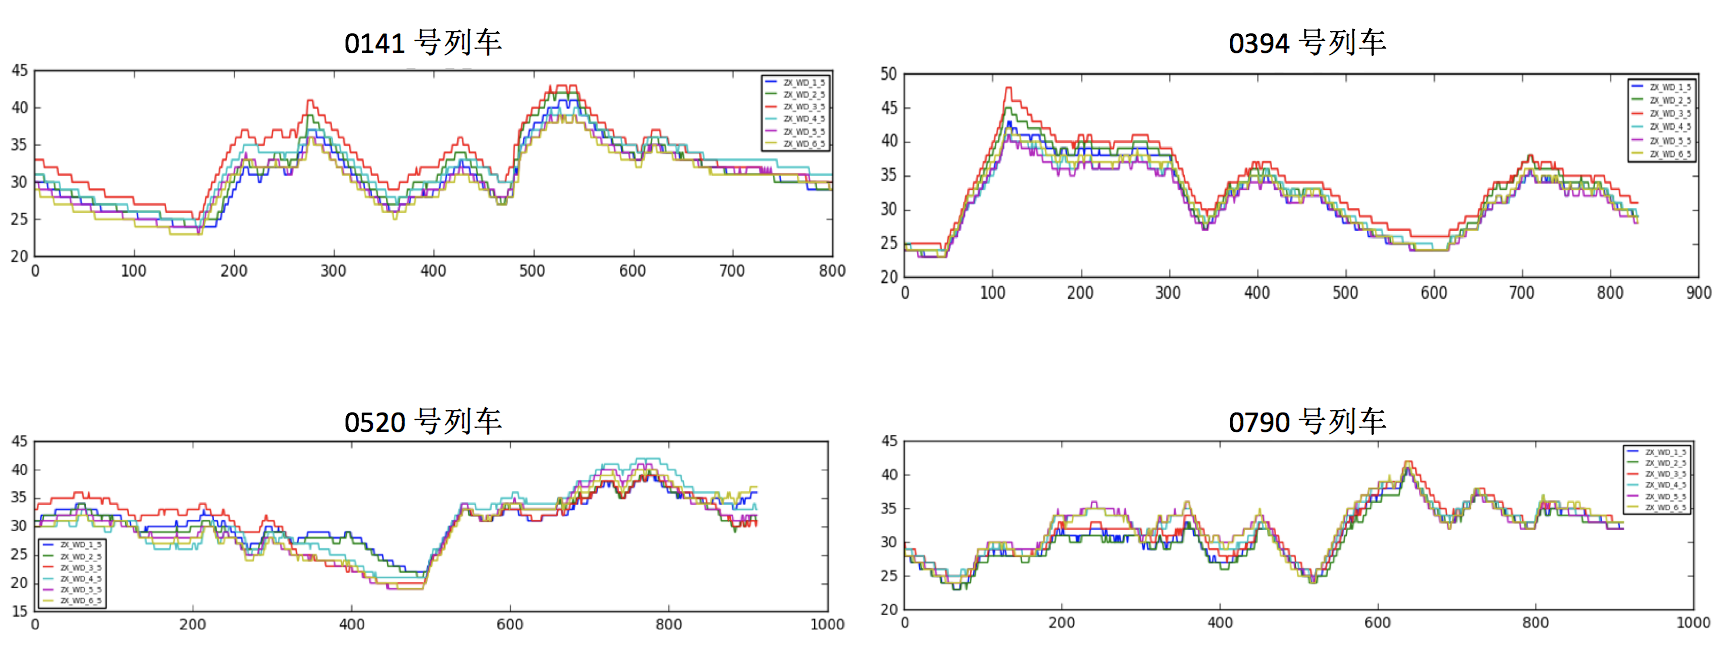
\includegraphics[scale=0.5]{figures/sr-data-temp.png}
\caption{不同高速列车不同观测点的温度数据}
\label{fig:sr-data-temp-corr}
\end{figure}  
(2)数据探索

本文对若干机车组三个月的温度数据进行探索分析,利用多种可视化方法或工具对数据进行理解、通过先进的时间序列分析方法探索温度数据的稳定性和相关性,具体方法细节参考\inlinecite{bisgaard2011time}。本文发现通过传感器采集的温度数据有以下特征:
\begin{itemize}
  \item 温度数据的采样率在1/10Hz到10Hz之间。
  \item 环境和车轴温度具有时变和不稳定的性质。事实上,轴承的内部动态性会根据不同的工作模式而改变。
  \item 轴承内部温度由\ref{eq:data-temp-generate}解析式决定\cite{陈德生2003列车轴温规律及红外线轴温探测方式的研究}。车轴的最大稳定温度为$t_{stable}$,由以下几个因素决定,车轴直径和车轮直径的比值 $(\frac{D_{axle}}{D_{wheel}})$,车轴盒压力 (\emph{P}),机车速度 (\emph{V}),摩擦因子(\emph{f}),和散热能力$(\sum {\alpha_{i}F_{i}})$的倒数。车轴盒表面的温度上升速度为\emph{m},由散热能力$(\sum {\alpha_{i}F_{i}})$和热吸收能力$\sum {C_{i}P_{i}}$的比值决定。$t_{raise}$表示温度上升遵循指数方程。
  \item 轴承内部状态通常无法直接探测。不同位置感知的温度数据由影响轴承状态的多种因素决定,包括但不仅限于机车的工作状态(比如,运行速度和牵引水平),传感器和轴承的相对位置,环境因素(比如环境温度和路线特点),以及其他多种外部干扰因素(比如空调系统的散热)。总的来说,来自不同传感器和/或不同车轴的数据存在强相关性但相关的模式会因工作状态的改变而变化。如图\ref{fig:sr-data-temp-corr}所示,不同列车的车轴温度数据形状各异,但不同轴位点之间的温度数据存在强相关性。
  \item 传感器数据存在高噪的特性。传感器工作过程中会受到多个噪音源的影响,比如来自车载空调系统的排气口的影响。
  \item 轴承失效模式具有高度复杂性。在当前的机车上,当传感器测量值超过预设预值时车载监控系统将产生失效报告。然而,这样基于域值的方案无法用于预防性维修。此外,一个固定的域值无法覆盖所有失效模式。事实上,温度梯度的上升和多种温度亚域值(sub-threshold)峰值可以反应系统失效。
\end{itemize}
\begin{equation}
\label{eq:data-temp-generate}
\left\{\begin{array}{l}
t_{stable} = \frac{D_{axle}\ast P\ast f \ast V}{D_{wheel}\ast \sum \alpha_{i}F_{i}}  \\[0.2cm]
t_{raise} = t_{stable}\ast (1-e^{-m\tau}) \\[0.2cm]
t_{sink} = t_{stable} \ast e^{-m\tau} \\[0.2cm]
m = \frac{\sum \alpha_{i}f_{i}}{\sum C_{i}P_{i}}
\end{array}\right.
\end{equation}

\section{模型与应用方案设计}

一方面,基于实际场景的考察和数据探索分析,有以下几点重要发现:(1)温度传感器已经得到了更广泛部署;(2)近年来已有重要的研究工作关注热轮轴温度的预测问题\cite{ma2016prediction,yi2015faults,amini2016wayside},在一定程度上说明温度数据对系统性能的敏感性;(3)高速列车组不同列车在不同运行环境下的车轴温度数据形状各异,但同一列车在一次运行中不同轴位点之间的温度数据存在强相关性。另一方面,本文通过领域专家和相关研究成果获知:工业系统的运作需要依赖一个或一组物理方程,工业时间序列普遍由潜在模型产生和控制\cite{bongard2007automated}。综合以上两方面,本文主要以多维车轴温度数据为基础,提出基于符号回归的系统动态方程学习框架,以理解系统的动态特性和各信号间的相互作用关系。进一步,基于系统方程构建时间序列预测模型以形成在线实时异常检测框架。

\label{sec:sr-model}
\subsection{基于符号回归的系统动态方程学习框架}

(1)符号和变量定义

\begin{itemize}

  \item 令小写字母黑体表示向量,即$\mathbf{a,b,c,d,...,x,y,z}$。

  \item 令大写字母黑体表示矩阵,即$\mathbf{A,B,C,D,...,X,Y,Z}$。

  \item 假设数据采样点为$\mathbf{t}=[t_{1},t_{2},...,t_{n}]$,以时间为单位非递减有序,默认等间隔。

  \item 假设一次采样结果为$(\mathbf{X},\mathbf{y})$,其中$\mathbf{X}$为{\heiti 因变量},$\mathbf{y}$为{\heiti 目标变量}。
  因变量$ \mathbf{X} \in R^{n\times m} $定义为\ref{equ:sr-object-func-x},是\emph{n}行和\emph{m}列矩阵,\emph{n}行表示对应$\mathbf{t}$的\emph{n}个时刻的观测结果,\emph{m}列表示\emph{m}个不同观测变量。
  目标变量$\mathbf{y}$定义为\ref{equ:sr-object-func-y},是对应$\mathbf{t}$的\emph{n}个时刻的观测结果。

  \item 假设有{\heiti 运算子}集合$\mathbf{P}$,定义如\ref{equ:sr-ops},其中每个元素表示一个基本的算数运算,对输入向量的每个元素进行相应的算数运算后返回结果向量。当前运算包括:
  加法运算$add(\mathbf{x,y})$表示两个输入向量的和,即返回$\mathbf{x}+\mathbf{y}$;
  减法运算$sub(\mathbf{x,y})$,表示两个输入向量的差,即返回$\mathbf{x}-\mathbf{y}$;
  乘法运算$mul(\mathbf{x,y})$,表示两个输入向量的点积,即返回$\mathbf{x} * \mathbf{y}$;
  除法运算$divide(\mathbf{x,y})$,表示两个输入向量的商,即返回$\mathbf{x}/\mathbf{y}$;
  正弦运算$sin(\mathbf{x})$,返回输入向量的正弦运算结果;
  余弦运算$cos(\mathbf{x})$,返回输入向量余弦运算结果;
  对数运算$log(\mathbf{x}, i) $,返回输入向量的对数运算即过,即返回$log_{i}(\mathbf{x})$;
  幂运算$pow(\mathbf{x}, i)$,返回输入向量的幂运算结果,即返回$\mathbf{x}^{i}$;
  取最大值运算$max(\mathbf{x})$,返回输入向量的最大值;
  取最小值运算$min(\mathbf{x})$,返回输入向量的最小值。
  \item 基函数向量$\mathbf{\Psi}$,定义如\ref{equ:sr-basefunc},一共有$n_{b}$个元素,其中每个元素$\varphi_{i}$表示一个{\heiti 基函数},基函数是由运算子集合$\mathbf{P}$中若干个运算子构成的线性或非线性复杂函数。

\end{itemize}
\begin{subequations}
\begin{align}
\mathbf{X} &= \begin{bmatrix}
x_{1}(t_{1}) & x_{2}(t_{1}) & ... & x_{m}(t_{1}) \\ 
x_{1}(t_{2}) & x_{2}(t_{2})  & ...  & x_{m}(t_{2}) \\ 
... & ... & ...  & ... \\ 
x_{1}(t_{n}) & x_{2}(t_{n})  & ...  & x_{m}(t_{n}) 
\end{bmatrix} = [x_{1}(\mathbf{t}), x_{2}(\mathbf{t}), ..., x_{m}(\mathbf{t})] = [\mathbf{x_{1}}, \mathbf{x_{2}}, ..., \mathbf{x_{m}}] \label{equ:sr-object-func-x} \\
\mathbf{y} &= [y(t_{1}), y(t_{2}), ..., y(t_{n})]^{T} \label{equ:sr-object-func-y}\\
\mathbf{\Psi} &= [\varphi_{1}, \varphi_{2}, ..., \varphi_{n_{b}}] \label{equ:sr-basefunc} \\
\mathbf{P} &= \begin{bmatrix}
add(\mathbf{x,y}) & sub(\mathbf{x,y}) & mul(\mathbf{x,y}) & divide(\mathbf{x,y}) \\ 
sin(\mathbf{x}) & cos(\mathbf{x}) & log(\mathbf{x}, i) & pow(\mathbf{x}, i) \\ 
max(\mathbf{x})& min(\mathbf{x}) & ... & ...  \\ 
\end{bmatrix} \label{equ:sr-ops} 
\end{align}
\end{subequations}

(2)基于符号回归的动态方程学习框架

图\ref{fig:sr-anomaly-framework}(左)是基于符号回归的系统动态特征学习框架,具体流程如下:
\begin{enumerate}[1.]
  \item 初始化:设定运算子集合$\mathbf{P}$,定义为\ref{equ:sr-ops},作为基函数集合$\mathbf{\Psi}$的初始值。输入因变量$\mathbf{X}$作为操作数,以及对应的目标变量$\mathbf{y}$作为评估指标计算的参考。
  \item 结构生成:基于某种算法从基函数集合$\mathbf{\Psi}$选择若干个基函数作为基本算子或操作数进行组合形成新的更复杂的基函数并将其加入到当前基函数集合中。由此循环迭代,通过某种度量指标控制基函数集合的大小和质量,当迭代触发某个域值时停止,并将基函数集合输入到下一环节。
  \item 参数学习:对输入的基函数集合$\mathbf{\Psi}$进行融合,即通过回归模型\ref{equ:sr-object-func}对目标变量进行估计,通过计算估计量$\mathbf{\hat{y}}$和实际观测量$\mathbf{y}$的误差来进行模型参数学习。即对模型\ref{equ:sr-object-func}的参数$\{a_{i}\},i=1,...,n_{b}$和$\mathbf{b}$进行学习。
  \item 模型选择:通过某种度量指标对模型$f(\mathbf{X})$的质量进行评价,从而作出是否接受当前学习结果的决策,若对学习结果不满意则返回第2步,甚至可以返回第1步对模型输入进行调整。若对学习结果满意,则将当前模型输出。
  \item 结束:最后框架的输出为一个或若干个优选的模型,定义为\ref{equ:sr-models},还会给出每个模型的评价指标。这些模型可以表达系统的底层动态特性和运行机理,还可以为后期其他任务提供支持,比如作为预测模型的基础。
\end{enumerate}
\begin{figure}[H]
\centering
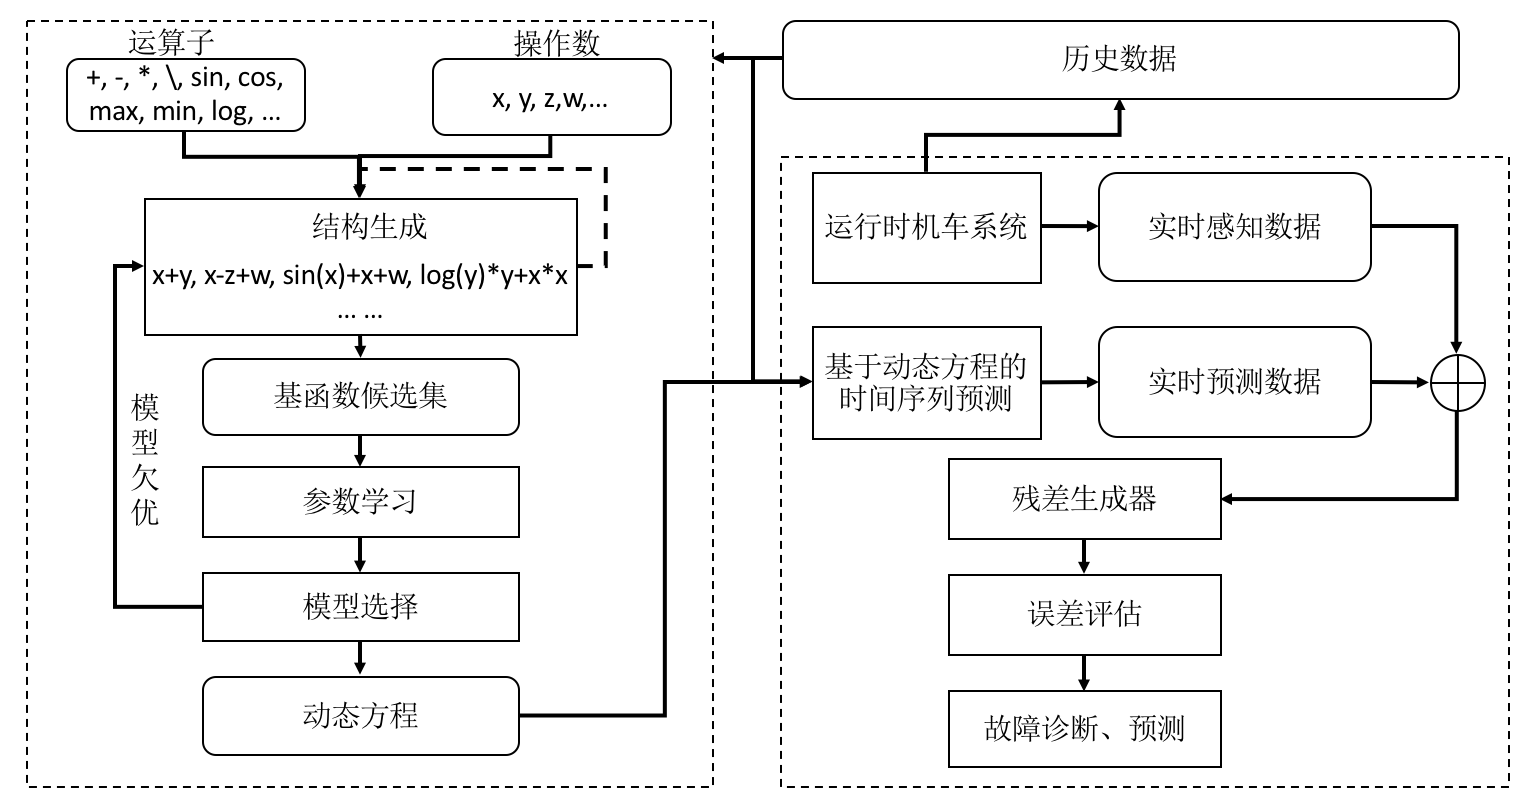
\includegraphics[scale=0.5]{figures/sr-anomaly-framework.png}
\caption{(左)基于符号回归的系统动态特征学习框架,(右)在线实时异常检测框架}
\label{fig:sr-anomaly-framework}
\end{figure}
\begin{subequations}
\begin{align}
\mathbf{\hat{y}} &= f(\mathbf{X}) = \mathbf{b} + \sum_{i=1}^{n_{b}}a_{i} \ast \mathbf{\Psi}_{i}(\mathbf{X}) =  \mathbf{b} + \sum_{i=1}^{n_{b}}a_{i} \ast \mathbf{\Psi}_{i}(\mathbf{\mathbf{x_{1}}, \mathbf{x_{2}}, ..., \mathbf{x_{m}}}) \label{equ:sr-object-func} \\
\mathbf{M} &= [f_{1}, f_{2}, ..., f_{n_m}] \label{equ:sr-models} 
\end{align}
\end{subequations}

(3)基于符号回归的系统动态特征学习框架的训练优化算法

本文融合 FFX\cite{mcconaghy2011ffx} 和 Deap\cite{fortin2012deap}作为框架中结构生成以及参数学习引擎。前者用于生成初始解,而后者则用于对FFX产生的结果进行修剪以形成更简化的模型。具体算法描述如下:

FFX 算法主要有以下 3 个步骤:
\begin{enumerate}[1.]
      \item 产生一个大规模的基函数集合。
      \item 识别最优的基函数并使用路径规整学习(pathwise regularized learning)进行参数学习。
      \item 通过最小化错误率和复杂度的目标过滤掉冗余候选函数。
\end{enumerate}
基于 Deap 遗传编程的符号回归循环执行以下3个步骤,直到收敛为止:
\begin{enumerate}[1.]
      \item 繁殖步:基于当前候选集产生新的候选集(即子孙)并通过突变和交叉操作保证种群的多样性。
      \item 评估步:对上一步产生的子孙进行评估。
      \item 选择步:基于上一步的评估结果选择优秀的子孙构成下一代的种群。
\end{enumerate}

(4)基于符号回归的系统动态特征学习框架的评价指标

1. 参数学习模块:本文基于误差平方和最小为目标,即最小化等式\ref{equ:sr-loss-rmse}。

2. 模型选择模块,不同于一般的回归方法,本文同时考虑模型准确率和模型可解释性,分别由准确率因子和理解性因子度量。准确率因定义为估计值和真实值的误差平方和,定义为等式\ref{equ:sr-loss-rmse}。理解性因子由模型规模度量,定义为\ref{equ:sr-loss-complexity},由基函数个数表示,基函数越多说明函数越复杂进而表明可解释性越差。综上可得最终的模型选择度量指标\ref{equ:sr-loss},其中参数$\lambda$用于平衡两个因素的重要程度。
\begin{subequations}
\begin{align}
L &= RMSE + \lambda C \label{equ:sr-loss} , \lambda \in [0,1]\\
RMSE &= \sqrt{\frac{\sum_{i=1}^{n} (\hat{y_{t_{i}}} - y_{t_{i}})^{2}}{n} } \label{equ:sr-loss-rmse} \\
C &= size(f(\mathbf{X})) \label{equ:sr-loss-complexity}
\end{align}
\end{subequations}

\subsection{基于系统动态方程的在线实时异常检测框架}
图\ref{fig:sr-anomaly-framework}为本文设计的故障诊断和预测框架。有以下几个核心内容:

(1) 实时数据采集

列车运行过程产生的数据主要通过传感器进行采集。有两个主要的数据流向,一方面,采集的数据将会被传输到数据中心的数据库中进行有效存储;另一方面,实时监测数据将会作为实时异常检测的基线。

(2) 实时异常检测
\begin{enumerate}[1.]
    \item 获取实时预测数据:通过基于符号回归的系统动态特征学习框架提供的最优系统动态方程$f_{best}$实现时间序列数据在线预测,即通过等式\ref{equ:sr-predict}来预测未来$w$个时刻内的监测数据轨迹$\mathbf{\hat{y}}$,$w$ 为给定的时间窗口。
    \item 获取实时感知数据:通过传感器获取最新的$w$个时刻内的实时监测数据$\mathbf{y}$。
    \item 残差生成:$\mathbf{\hat{y}}$和$\mathbf{y}$被同时输送到残差生成器,残差生成器通过等式\ref{equ:sr-residual}计算系统实时误差。
    \item 残差评估:残差评估的方法多样,本文采用平均误差进行评价,定义为\ref{equ:sr-metrics},主要基于以下考虑:(1)由轴承内部温度解析式\ref{eq:data-temp-generate}可知,系统失效时轴承温度升高$t_{raise}$遵循指数方程,预测值和真实值之间的平均误差已经足以在要求时间内发现故障;(2)整个在线异常框架需要满足实时计算要求,而目前的实际项目平台仍有待进一步升级,难以支持过于复杂的评估方法。
    \item 故障诊断和预测:基于残差评估的结果,本文通过等式\ref{equ:sr-loss-alarm}作出是否报警的决策,其中$\alpha$为报警域值,根据实际应用需求而定。
\end{enumerate}

(3) 在线模型定期更新

基于符号回归的系统动态特征学习框架,如图\ref{fig:sr-anomaly-framework}(左),会从数据中心的数据库中获取最新的历史数据对在线模型进行定期更新,使在线模型具有对复杂环境的自适应能力,形成了整个异常检测框架的闭环。值得注意的是,动态方程学习过程为离线完成不影响在线异常检测框架的效率。在给定系统方程时计算速度很快可实现实时预测。
%整个在线框架的时间瓶颈主要在于传输延时,这是整个实际项目的系统化工程,本文不作展开。
\begin{subequations}
\begin{align}
\mathbf{\hat{y}} &= f_{best}(\mathbf{X}) = [y_{t_{1}}, y_{t_{2}}, ..., y_{t_{w}}] \label{equ:sr-predict}\\
\mathbf{r} &= \hat{\mathbf{y}_{t_{i}}} - \mathbf{y}_{t_{i}}, i=1,2,...,w \label{equ:sr-residual} \\
\gamma  &= \sqrt{\frac{\sum_{i=1}^{w} \mathbf{r}_{i}^{2}}{w} } \label{equ:sr-metrics} \\
alarm &= \begin{cases}
 1 &  \gamma \geqslant \alpha   \\ 
 0 &   \gamma  < \alpha
\end{cases} \label{equ:sr-loss-alarm}
\end{align}
\end{subequations}

\section{实验结果及分析}
\label{sec:sr-experiment}

本文通过符号回归的逆向工程技术揭示 6 个高速列车走行部轴温的动态性,6 个轴温的标号为 ZX\_WD\_1,ZX\_WD\_2,ZX\_WD\_3,ZX\_WD\_4,ZX\_WD\_5,ZX\_WD\_6。此外还考虑了 ZX\_HW\_1, ZX\_HW\_2, ZD\_LCG, ZD\_TFG, ZD\_JHG, ZD\_LLJ, ZD\_SPEED,变量的定义和说明见表\ref{tab:sr-variables}。本文在 1000 次运行过程中采集的数据集上进行交叉验证。表\ref{tab:sr-ffx-1}至表\ref{tab:sr-ffx-6}给出了FFX的学习结果,表\ref{tab:sr-deap-1}至表\ref{tab:sr-deap-6}给出了对应的经过基于遗传编程算法剪枝以后结果。图\ref{fig:ffx_zx_wd}给出了基于FFX的动态方程估计数据和原数据的对比结果,图\ref{fig:deap_zx_wd}给出了基于遗传编程算法剪枝以后的动态方程估计数据和原数据的对比结果。以上结果充分说明本文的符号回归方法可以有效揭示高速列车走行部轴温正常和失效状态下的动态特性,并且简洁的动态方程对真实数据的拟合效果很好。本章节的分析框架已通过机车监控中心进行实时测试。

\begin{figure}[H]
\centering
\begin{subfigure}[t]{0.48\textwidth}
    \centering
    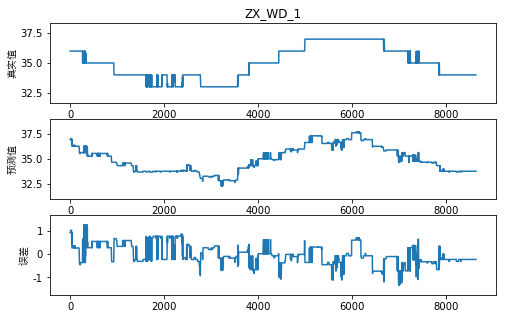
\includegraphics[scale=0.45]{figures/sr/ffx-zx_wd_1.png}
    %\caption{ZX\_WD\_1}
\end{subfigure}\hfill
\begin{subfigure}[t]{0.48\textwidth}
    \centering
    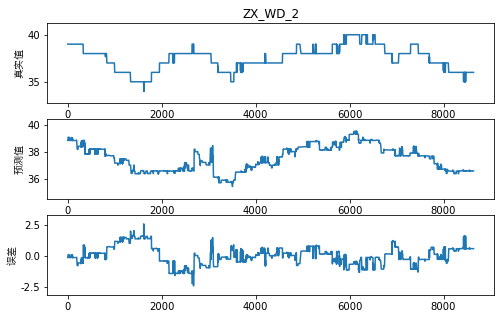
\includegraphics[scale=0.45]{figures/sr/ffx-zx_wd_2.png}
    %\caption{ZX\_WD\_2}
\end{subfigure}\\
\begin{subfigure}[t]{0.48\textwidth}
  \centering
  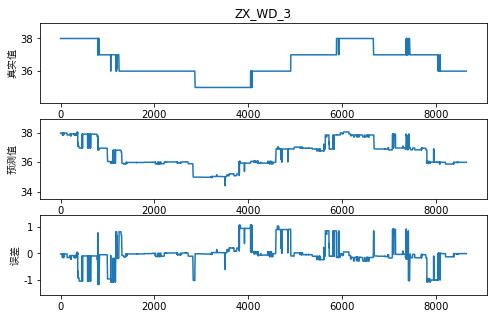
\includegraphics[scale=0.45]{figures/sr/ffx-zx_wd_3.png}
  %\caption{ZX\_WD\_3}
\end{subfigure}\hfill
\begin{subfigure}[t]{0.48\textwidth}
    \centering
    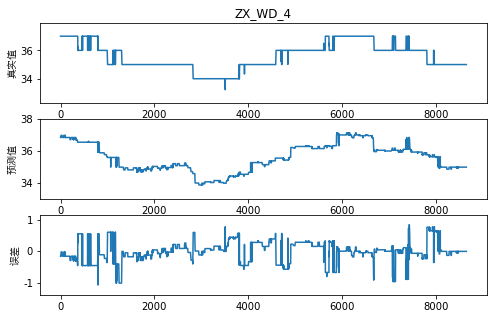
\includegraphics[scale=0.45]{figures/sr/ffx-zx_wd_4.png}
    %\caption{ZX\_WD\_4}
\end{subfigure}\\
\begin{subfigure}[t]{0.48\textwidth}
  \centering
  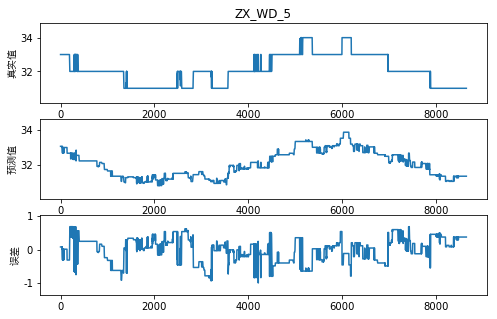
\includegraphics[scale=0.45]{figures/sr/ffx-zx_wd_5.png}
  %\caption{ZX\_WD\_5}
\end{subfigure}\hfill
\begin{subfigure}[t]{0.48\textwidth}
    \centering
    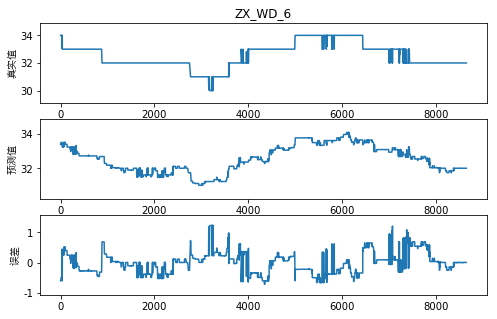
\includegraphics[scale=0.45]{figures/sr/ffx-zx_wd_6.png}
    %\caption{ZX\_WD\_6}
\end{subfigure}
\caption{ffx-轴承温度的预测结果}
\label{fig:ffx_zx_wd}
\end{figure}
\begin{longtable}[c]{p{9cm}*{3}{l}}
\caption{基于FFX学习的揭示ZX\_WD\_1动态特征性能最好的前8个方程}\label{tab:sr-ffx-1}\\
\toprule[1.5pt]
模型 & 测试误差 & 训练误差 & 复杂度 \\\midrule[1pt]
\endfirsthead
\multicolumn{4}{l}{续表~\thetable\hskip1em 基于FFX学习的揭示ZX\_WD\_1动态特征性能最好的前8个方程}\\
\toprule[1.5pt]
模型 & 测试误差 & 训练误差 & 复杂度 \\\midrule[1pt]
\endhead
\hline
\multicolumn{4}{r}{续下页}
\endfoot
\endlastfoot
      35.0 & 1.354576 & 1.355095 & 0 \\
      25.5 + 0.00904*ZX\_WD\_5 * ZX\_WD\_6 & 0.913770 & 0.914579 & 1 \\
      8.74 + 0.519*ZX\_WD\_6 + 0.291*ZX\_WD\_5 & 0.753903 & 0.754591 & 2 \\
      6.03 + 0.539*ZX\_WD\_6 + 0.332*ZX\_WD\_5 + 0.0223*ZX\_HW\_2 & 0.694735 & 0.695431 & 3 \\
      14.2 / (1.0 - 0.00703*ZX\_WD\_6 - 0.00690*ZX\_WD\_5 - 0.00302*ZX\_WD\_4 - 0.00103*ZX\_HW\_2) & 0.427490 & 0.427225 & 4 \\
      (14.6 - 0.0243*ZX\_HW\_1) / (1.0 - 0.00706*ZX\_WD\_5 - 0.00704*ZX\_WD\_6 - 0.00297*ZX\_WD\_4 - 0.00125*ZX\_HW\_2) & 0.421005 & 0.420607 & 5 \\
      -42.2 + 13.4*log10(ZX\_WD\_5) * log10(ZX\_WD\_6) + 9.72*log10(ZX\_WD\_5) * log10(ZX\_WD\_4) + 8.08*log10(ZX\_WD\_5) * log10(ZX\_HW\_2) + 0.691*log10(ZX\_WD\_2) * log10(ZX\_WD\_6) + 0.00511*ZX\_WD\_6\^2 - 0.00176*ZX\_HW\_1\^2 & 0.409125 & 0.409015 & 6 \\ 
      32.6 - 0.557*max(0,33.2-ZX\_WD\_5) + 0.255*max(0,ZX\_WD\_6-31.3) - 0.235*max(0,36.0-ZX\_WD\_4) + 0.212*max(0,ZX\_WD\_6-30.8) - 0.131*max(0,36.1-ZX\_HW\_2) + 0.101*max(0,ZX\_WD\_5-32.0) + 0.0911*max(0,ZX\_WD\_6-31.9) + 0.0778*ZX\_WD\_6 + 0.0591*max(0,ZX\_WD\_2-37.6) & 0.397894 & 0.398467 & 9 \\
\bottomrule[1.5pt]
\end{longtable}
\begin{longtable}[c]{p{9cm}*{3}{l}}
\caption{基于FFX学习的揭示ZX\_WD\_2动态特征性能最好的前8个方程}\label{tab:sr-ffx-2}\\
\toprule[1.5pt]
模型 & 测试误差 & 训练误差 & 复杂度 \\\midrule[1pt]
\endfirsthead
\multicolumn{4}{l}{续表~\thetable\hskip1em 基于FFX学习的揭示ZX\_WD\_2动态特征性能最好的前8个方程}\\
\toprule[1.5pt]
模型 & 测试误差 & 训练误差 & 复杂度 \\\midrule[1pt]
\endhead
\hline
\multicolumn{4}{r}{续下页}
\endfoot
\endlastfoot
      37.5 & 1.249001 & 1.249430 & 0 \\
      33.6 + 0.00339*ZX\_WD\_4 * ZX\_WD\_5 & 1.114234 & 1.114899 & 1 \\
      22.5 + 0.00923*ZX\_WD\_4 * ZX\_WD\_5 + 0.00380*ZX\_WD\_3 * ZX\_WD\_5 & 0.842994 & 0.844262 & 2 \\
      17.9 / (1.0 - 0.00748*ZX\_WD\_5 - 0.00444*ZX\_WD\_4 - 0.00341*ZX\_WD\_3) & 0.806176 & 0.807632 & 3 \\
      20.9 + 0.00870*ZX\_WD\_4 * ZX\_WD\_5 + 0.00399*ZX\_WD\_3 * ZX\_WD\_5 + 0.00286*ZX\_WD\_4 * ZX\_HW\_2 - 3.78e-6*ZD\_TFG\^2 & 0.757751 & 0.759322 & 4 \\
      -15.2 + 13.8*log10(ZX\_WD\_5) * log10(ZX\_WD\_4) + 7.53*log10(ZX\_WD\_5) * log10(ZX\_WD\_3) + 0.00250*ZX\_HW\_2\^2 + 0.00147*ZX\_WD\_4\^2 - 5.22e-6*ZD\_TFG\^2 & 0.740418 & 0.741918 & 5 \\
      -14.2 + 13.1*log10(ZX\_WD\_5) * log10(ZX\_WD\_4) + 7.59*log10(ZX\_WD\_5) * log10(ZX\_WD\_3) + 0.00293*ZX\_HW\_2\^2 + 0.00163*ZX\_WD\_4\^2 - 0.000125*ZD\_JHG - 5.62e-6*ZD\_TFG\^2 & 0.734446 & 0.735908 & 6 \\
      20.5 + 0.00813*ZX\_WD\_4 * ZX\_WD\_5 + 0.00373*ZX\_WD\_3 * ZX\_WD\_5 + 0.00320*ZX\_WD\_4 * ZX\_HW\_2 + 0.00108*ZX\_HW\_2\^2 + 0.000383*ZX\_WD\_3 * ZX\_HW\_2 - 0.000157*ZD\_JHG - 5.69e-6*ZD\_TFG\^2 & 0.731474 & 0.732970 & 7 \\ 
\bottomrule[1.5pt]
\end{longtable}
\begin{longtable}[c]{p{9cm}*{3}{l}}
\caption{基于FFX学习的揭示ZX\_WD\_3动态特征性能最好的前8个方程}\label{tab:sr-ffx-3}\\
\toprule[1.5pt]
模型 & 测试误差 & 训练误差 & 复杂度 \\\midrule[1pt]
\endfirsthead
\multicolumn{4}{l}{续表~\thetable\hskip1em 基于FFX学习的揭示ZX\_WD\_3动态特征性能最好的前8个方程}\\
\toprule[1.5pt]
模型 & 测试误差 & 训练误差 & 复杂度 \\\midrule[1pt]
\endhead
\hline
\multicolumn{4}{r}{续下页}
\endfoot
\endlastfoot
      36.6 & 0.949297 & 0.949557 & 0 \\
      6.55 + 0.843*ZX\_WD\_4 & 0.402844 & 0.401142 & 1 \\
      4.39 + 0.878*ZX\_WD\_4 + 0.0282*ZX\_HW\_1 & 0.395118 & 0.393432 & 2 \\
      (19.0 - 0.00995*ZX\_WD\_5) / (1.0 - 0.0125*ZX\_WD\_4 - 0.00135*ZX\_HW\_1) & 0.393192 & 0.391551 & 3 \\
      (19.4 - 0.0342*ZX\_WD\_5) / (1.0 - 0.0123*ZX\_WD\_4 - 0.00169*ZX\_HW\_1 - 0.000162*ZX\_WD\_2) & 0.389710 & 0.388109 & 4 \\
      4.12 + 0.891*ZX\_WD\_4 + 0.0744*ZX\_HW\_1 - 0.0733*ZX\_WD\_5 + 0.0177*ZX\_WD\_2 - 0.00114*ZD\_LLJ & 0.386751 & 0.385115 & 5 \\
      17.7 / (1.0 - 0.0122*ZX\_WD\_4 - 0.00192*ZX\_HW\_1 - 0.00125*max(0,33.6-ZX\_WD\_5) - 0.000561*max(0,35.9-ZX\_WD\_1) - 0.000312*ZX\_WD\_2 - 0.000132*ZX\_WD\_6) & 0.385381 & 0.383703 & 6 \\
      3.51 + 0.920*ZX\_WD\_4 + 0.126*ZX\_HW\_1 - 0.120*ZX\_WD\_5 + 0.0374*ZX\_WD\_2 - 0.0306*ZX\_HW\_2 - 0.00734*ZX\_WD\_1 - 0.00178*ZD\_LLJ & 0.381686 & 0.380206 & 7 \\
\bottomrule[1.5pt]
\end{longtable}
\begin{longtable}[c]{p{9cm}*{3}{l}}
\caption{基于FFX学习的揭示ZX\_WD\_4动态特征性能最好的前8个方程}\label{tab:sr-ffx-4}\\
\toprule[1.5pt]
模型 & 测试误差 & 训练误差 & 复杂度 \\\midrule[1pt]
\endfirsthead
\multicolumn{4}{l}{续表~\thetable\hskip1em 基于FFX学习的揭示ZX\_WD\_4动态特征性能最好的前8个方程}\\
\toprule[1.5pt]
模型 & 测试误差 & 训练误差 & 复杂度 \\\midrule[1pt]
\endhead
\hline
\multicolumn{4}{r}{续下页}
\endfoot
\endlastfoot
     35.6 & 0.930301 & 0.931435 & 0 \\
      23.4 + 0.333*ZX\_WD\_3 & 0.656427 & 0.657099 & 1 \\
      21.0 + 0.218*ZX\_WD\_3 * log10(ZX\_WD\_1) + 0.00185*ZX\_HW\_2 * ZX\_WD\_3 & 0.453389 & 0.453613 & 2 \\
      16.3 + 0.260*ZX\_WD\_3 * log10(ZX\_WD\_1) + 0.00299*ZX\_HW\_2 * ZX\_WD\_3 + 0.000653*ZX\_WD\_3\^2 & 0.335498 & 0.335179 & 3 \\
      3.34 + 0.610*ZX\_WD\_3 + 0.124*ZX\_HW\_2 + 0.108*ZX\_WD\_1 + 0.0504*ZX\_WD\_2 & 0.308872 & 0.308640 & 4 \\
      13.0 + 1.68*log10(ZX\_WD\_3) * log10(ZX\_WD\_1) + 0.173*ZX\_WD\_3 * log10(ZX\_WD\_1) + 0.00352*ZX\_HW\_2 * ZX\_WD\_3 + 0.00258*ZX\_WD\_3\^2 + 0.000618*ZX\_WD\_2\^2 & 0.308366 & 0.308182 & 5 \\
      3.26 + 0.616*ZX\_WD\_3 + 0.132*ZX\_HW\_2 + 0.113*ZX\_WD\_1 + 0.0526*ZX\_WD\_2 - 0.0209*ZX\_HW\_1 + 0.000356*ZD\_LLJ & 0.307278 & 0.307066 & 6 \\
      3.36 + 0.621*ZX\_WD\_3 + 0.143*ZX\_HW\_2 + 0.117*ZX\_WD\_1 + 0.0538*ZX\_WD\_2 - 0.0464*ZX\_HW\_1 - 0.000745*ZD\_SPEED + 0.000611*ZD\_LLJ & 0.306412 & 0.306220 & 7 \\
\bottomrule[1.5pt]
\end{longtable}
\begin{longtable}[c]{p{9cm}*{3}{l}}
\caption{基于FFX学习的揭示ZX\_WD\_5动态特征性能最好的前8个方程}\label{tab:sr-ffx-5}\\
\toprule[1.5pt]
模型 & 测试误差 & 训练误差 & 复杂度 \\\midrule[1pt]
\endfirsthead
\multicolumn{4}{l}{续表~\thetable\hskip1em 基于FFX学习的揭示ZX\_WD\_5动态特征性能最好的前8个方程}\\
\toprule[1.5pt]
模型 & 测试误差 & 训练误差 & 复杂度 \\\midrule[1pt]
\endhead
\hline
\multicolumn{4}{r}{续下页}
\endfoot
\endlastfoot
     32.1 & 0.868038 & 0.867657 & 0 \\
      22.2 + 0.283*ZX\_WD\_1 & 0.571645 & 0.571623 & 1 \\
      18.5 + 0.330*ZX\_WD\_1 + 0.0625*ZX\_HW\_1 & 0.503551 & 0.503674 & 2 \\
      18.3 / (1.0 - 0.00542*ZX\_WD\_1 - 0.00493*ZX\_HW\_1 - 0.00213*ZX\_WD\_2) & 0.409921 & 0.410352 & 3 \\
      31.4 + 0.316*max(0,ZX\_WD\_1-33.8) + 0.141*max(0,ZX\_HW\_1-32.3) + 0.129*max(0,ZX\_WD\_1-34.3) + 0.121*max(0,ZX\_HW\_1-31.8) & 0.398462 & 0.398821 & 4 \\
      31.4 + 0.318*max(0,ZX\_WD\_1-33.8) + 0.222*max(0,ZX\_HW\_1-32.3) + 0.145*max(0,ZX\_WD\_1-34.3) + 0.0893*max(0,ZX\_HW\_1-31.8) - 0.0554*max(0,36.8-ZX\_WD\_2) & 0.377175 & 0.377608 & 5 \\
      17.3 / (1.0 - 0.00577*ZX\_WD\_1 - 0.00521*ZX\_HW\_1 - 0.00403*max(0,35.0-ZX\_WD\_4) - 0.00299*max(0,33.3-ZX\_HW\_2) - 0.00143*ZX\_WD\_2 - 0.00107*ZX\_WD\_6) & 0.354132 & 0.354684 & 6 \\
      31.4 + 0.342*max(0,ZX\_WD\_1-33.8) + 0.223*max(0,ZX\_HW\_1-32.3) + 0.146*max(0,32.3-ZX\_HW\_2) + 0.118*max(0,ZX\_HW\_1-31.8) + 0.106*max(0,ZX\_WD\_1-34.3) - 0.0740*max(0,36.8-ZX\_WD\_2) + 0.0600*max(0,35.0-ZX\_WD\_4) - 0.0396*max(0,36.5-ZX\_WD\_1) & 0.349669 & 0.350131 & 8 \\
\bottomrule[1.5pt]
\end{longtable}
\begin{longtable}[c]{p{9cm}*{3}{l}}
\caption{基于FFX学习的揭示ZX\_WD\_6动态特征性能最好的前8个方程}\label{tab:sr-ffx-6}\\
\toprule[1.5pt]
模型 & 测试误差 & 训练误差 & 复杂度 \\\midrule[1pt]
\endfirsthead
\multicolumn{4}{l}{续表~\thetable\hskip1em 基于FFX学习的揭示ZX\_WD\_6动态特征性能最好的前8个方程}\\
\toprule[1.5pt]
模型 & 测试误差 & 训练误差 & 复杂度 \\\midrule[1pt]
\endhead
\hline
\multicolumn{4}{r}{续下页}
\endfoot
\endlastfoot
    32.5 & 0.895700 & 0.895482 & 0 \\
      24.2 + 0.239*ZX\_WD\_1 & 0.619888 & 0.619435 & 1 \\
      20.2 + 0.300*ZX\_WD\_1 + 0.0527*ZX\_HW\_2 & 0.511317 & 0.510716 & 2 \\
      11.3 + 0.388*ZX\_WD\_1 + 0.122*ZX\_HW\_1 + 0.108*ZX\_HW\_2 & 0.363861 & 0.362749 & 3 \\
      8.84 + 0.404*ZX\_WD\_1 + 0.147*ZX\_HW\_1 + 0.112*ZX\_HW\_2 + 0.0257*ZX\_WD\_3 & 0.351119 & 0.350121 & 4 \\
      20.6 + 0.00430*ZX\_HW\_1 * ZX\_WD\_1 + 0.00323*ZX\_HW\_2 * ZX\_WD\_1 + 0.00161*ZX\_WD\_1\^2 + 0.000915*ZX\_WD\_3 * ZX\_WD\_1 + 4.54e-8*ZD\_JHG\^2 & 0.350564 & 0.349649 & 5 \\
      8.45 + 0.407*ZX\_WD\_1 + 0.152*ZX\_HW\_1 + 0.110*ZX\_HW\_2 + 0.0309*ZX\_WD\_3 + 0.000971*ZD\_SPEED + 0.000796*ZD\_LLJ & 0.349222 & 0.348054 & 6 \\
      8.37 + 5.21*log10(ZX\_HW\_1) * log10(ZX\_HW\_2) + 2.64*log10(ZX\_HW\_1) * log10(ZX\_WD\_3) - 0.959*log10(ZX\_WD\_2) + 0.00596*ZX\_WD\_1\^2 + 0.00206*ZD\_SPEED + 0.00197*ZD\_LLJ + 2.25e-7*ZD\_LCG\^2 & 0.344627 & 0.343397 & 7 \\
\bottomrule[1.5pt]
\end{longtable}
\begin{figure}[H]
\centering
\begin{subfigure}[t]{0.48\textwidth}
    \centering
    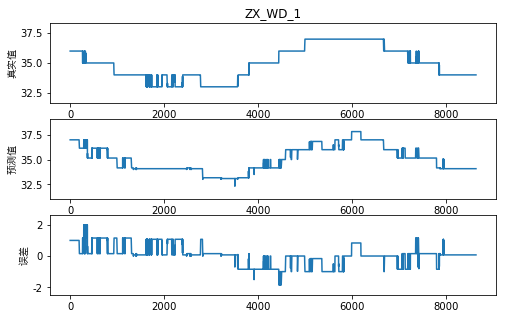
\includegraphics[scale=0.45]{figures/sr/deap-zw_wd_1.png}
    %%\caption{ZX\_WD\_1}
\end{subfigure}\hfill
\begin{subfigure}[t]{0.48\textwidth}
    \centering
    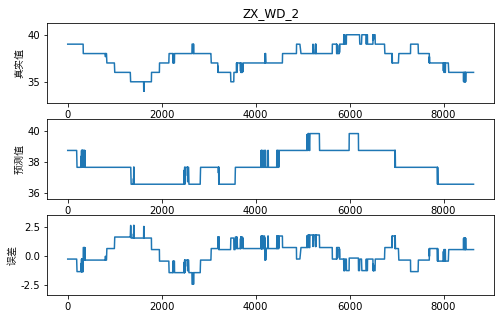
\includegraphics[scale=0.45]{figures/sr/deap-zw_wd_2.png}
    %%\caption{ZX\_WD\_2}
\end{subfigure}\\
\begin{subfigure}[t]{0.48\textwidth}
  \centering
  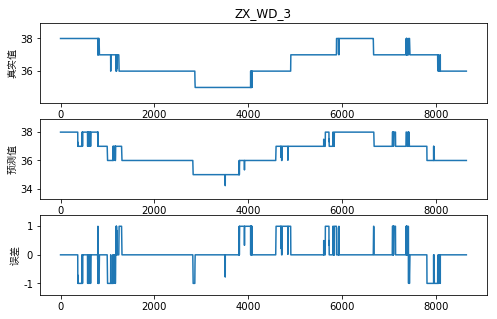
\includegraphics[scale=0.45]{figures/sr/deap-zw_wd_3.png}
  %%\caption{ZX\_WD\_3}
\end{subfigure}\hfill
\begin{subfigure}[t]{0.48\textwidth}
    \centering
    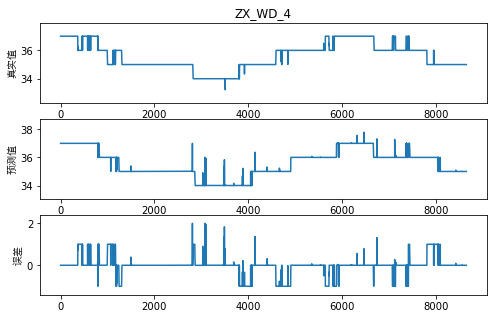
\includegraphics[scale=0.45]{figures/sr/deap-zw_wd_4.png}
    %%\caption{ZX\_WD\_4}
\end{subfigure}\\
\begin{subfigure}[t]{0.48\textwidth}
  \centering
  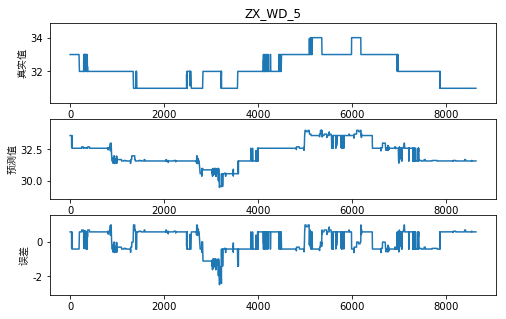
\includegraphics[scale=0.45]{figures/sr/deap-zw_wd_5.png}
  %%\caption{ZX\_WD\_5}
\end{subfigure}\hfill
\begin{subfigure}[t]{0.48\textwidth}
    \centering
    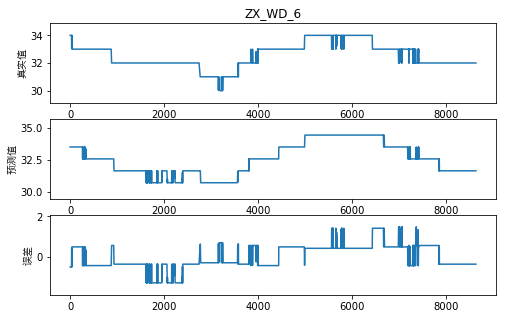
\includegraphics[scale=0.45]{figures/sr/deap-zw_wd_6.png}
    %%\caption{ZX\_WD\_6}
\end{subfigure}
\caption{deap-轴承温度的预测结果}
\label{fig:deap_zx_wd}
\end{figure}
\begin{longtable}[c]{p{4.3cm}p{4.3cm}*{3}{l}}
\caption{基于Deep剪枝后得到的揭示ZX\_WD\_1动态特征性能最好的方程}\label{tab:sr-deap-1}\\
\toprule[1.5pt]
原模型 & 简化模型 & 测试误差 & 训练误差 &  复杂度\\\midrule[1pt]
\endfirsthead
\multicolumn{5}{l}{续表~\thetable\hskip1em 基于Deep剪枝后得到的揭示ZX\_WD\_1动态特征性能最好的方程}\\
\toprule[1.5pt]
原模型 & 简化模型 & 测试误差 & 训练误差 &  复杂度 \\\midrule[1pt]
\endhead
\hline
\multicolumn{5}{r}{续下页}
\endfoot
\endlastfoot
      sqrt(ZD\_TFG) & sqrt(ZD\_TFG) & 10.039514 & 10.036110 & 2 \\
      Add(2.4220000000000002, ZX\_WD\_6) & ZX\_WD\_6 + 2.4220000000000002 & 0.670062 & 0.670128 & 3 \\
      Sub(ZX\_WD\_4, cos(ZX\_WD\_5)) & ZX\_WD\_4 - cos(ZX\_WD\_5) & 0.643303 & 0.642128 & 4 \\
\bottomrule[1.5pt]
\end{longtable}
\begin{longtable}[c]{p{4.3cm}p{4.3cm}*{3}{l}}
\caption{基于Deep剪枝后得到的揭示ZX\_WD\_2动态特征性能最好的方程}\label{tab:sr-deap-2}\\
\toprule[1.5pt]
原模型 & 简化模型 & 测试误差 & 训练误差 &  复杂度\\\midrule[1pt]
\endfirsthead
\multicolumn{5}{l}{续表~\thetable\hskip1em 基于Deep剪枝后得到的揭示ZX\_WD\_2动态特征性能最好的方程}\\
\toprule[1.5pt]
原模型 & 简化模型 & 测试误差 & 训练误差 &  复杂度 \\\midrule[1pt]
\endhead
\hline
\multicolumn{5}{r}{续下页}
\endfoot
\endlastfoot
      sqrt(ZD\_TFG) & sqrt(ZD\_TFG) & 12.576153 & 12.572426 & 2 \\
      Add(1.0, ZX\_WD\_3) & ZX\_WD\_3 + 1.0 & 0.981440 & 0.981503 & 3 \\
      Add(ZX\_WD\_3, 1.0) & ZX\_WD\_3 + 1.0 & 0.981440 & 0.981503 & 3 \\
      Add(ZX\_WD\_5, sqrt(ZX\_WD\_5)) & sqrt(ZX\_WD\_5) + ZX\_WD\_5 & 0.953105 & 0.953624 & 4 \\
      Add(sqrt(ZX\_WD\_5), ZX\_WD\_5) & sqrt(ZX\_WD\_5) + ZX\_WD\_5 & 0.953105 & 0.953624 & 4 \\
\bottomrule[1.5pt]
\end{longtable}

\begin{longtable}[c]{p{4.3cm}p{4.3cm}*{3}{l}}
\caption{基于Deep剪枝后得到的揭示ZX\_WD\_3动态特征性能最好的方程}\label{tab:sr-deap-3}\\
\toprule[1.5pt]
原模型 & 简化模型 & 测试误差 & 训练误差 &  复杂度\\\midrule[1pt]
\endfirsthead
\multicolumn{5}{l}{续表~\thetable\hskip1em 基于Deep剪枝后得到的揭示ZX\_WD\_3动态特征性能最好的方程}\\
\toprule[1.5pt]
原模型 & 简化模型 & 测试误差 & 训练误差 &  复杂度 \\\midrule[1pt]
\endhead
\hline
\multicolumn{5}{r}{续下页}
\endfoot
\endlastfoot
      sqrt(ZD\_TFG) & sqrt(ZD\_TFG) & 11.578368 & 11.573686 & 2 \\
      Add(ZX\_WD\_4, 1.0) & ZX\_WD\_4 + 1.0 & 0.402275 & 0.400682 & 3 \\
      Add(1.0, ZX\_WD\_4) & ZX\_WD\_4 + 1.0 & 0.402275 & 0.400682 & 3 \\
\bottomrule[1.5pt]
\end{longtable}
\begin{longtable}[c]{p{4.3cm}p{4.3cm}*{3}{l}}
\caption{基于Deep剪枝后得到的揭示ZX\_WD\_4动态特征性能最好的方程}\label{tab:sr-deap-4}\\
\toprule[1.5pt]
原模型 & 简化模型 & 测试误差 & 训练误差 &  复杂度\\\midrule[1pt]
\endfirsthead
\multicolumn{5}{l}{续表~\thetable\hskip1em 基于Deep剪枝后得到的揭示ZX\_WD\_4动态特征性能最好的方程}\\
\toprule[1.5pt]
原模型 & 简化模型 & 测试误差 & 训练误差 &  复杂度 \\\midrule[1pt]
\endhead
\hline
\multicolumn{5}{r}{续下页}
\endfoot
\endlastfoot
      sqrt(ZD\_TFG) & sqrt(ZD\_TFG) & 10.619709 & 10.616273 & 2 \\
      Add(3.0449999999999999, ZX\_WD\_6) & ZX\_WD\_6 + 3.0449999999999999 & 0.633333 & 0.633819 & 3 \\
      sqrt(Mul(ZX\_WD\_3, ZX\_HW\_2)) & sqrt(ZX\_HW\_2*ZX\_WD\_3) & 0.435390 & 0.435666 & 4 \\
      Add(cos(log(ZX\_WD\_3)), ZX\_WD\_3) & ZX\_WD\_3 + cos(log(ZX\_WD\_3)) & 0.409323 & 0.407365 & 5 \\
      Sub(ZX\_WD\_3, cos(Div(ZX\_WD\_3, ZD\_JHG))) & ZX\_WD\_3 - cos(ZX\_WD\_3/ZD\_JHG) & 0.407747 & 0.403063 & 6 \\
\bottomrule[1.5pt]
\end{longtable}
\begin{longtable}[c]{p{5cm}p{4.3cm}*{3}{c}}
\caption{基于Deep剪枝后得到的揭示ZX\_WD\_5动态特征性能最好的方程}\label{tab:sr-deap-5}\\
\toprule[1.5pt]
原模型 & 简化模型 & 测试误差 & 训练误差 &  复杂度\\\midrule[1pt]
\endfirsthead
\multicolumn{5}{l}{续表~\thetable\hskip1em 基于Deep剪枝后得到的揭示ZX\_WD\_5动态特征性能最好的方程}\\
\toprule[1.5pt]
原模型 & 简化模型 & 测试误差 & 训练误差 &  复杂度 \\\midrule[1pt]
\endhead
\hline
\multicolumn{5}{r}{续下页}
\endfoot
\endlastfoot
      sqrt(ZD\_TFG) & sqrt(ZD\_TFG) & 7.196478 & 7.190211 & 2 \\
      Add(-0.46400000000000002, ZX\_WD\_6) & ZX\_WD\_6 - 0.46400000000000002 & 0.607207 & 0.607687 & 3 \\
      Add(ZX\_WD\_6, log(cos(sin(log(cos(ZD\_TFG)))))) & ZX\_WD\_6 + log(cos(sin(log(cos(ZD\_TFG))))) & 0.594462 & 0.595329 & 9 \\
\bottomrule[1.5pt]
\end{longtable}
\begin{longtable}[c]{p{4cm}p{5.2cm}*{3}{c}}
\caption{基于Deep剪枝后得到的揭示ZX\_WD\_6动态特征性能最好的方程}\label{tab:sr-deap-6}\\
\toprule[1.5pt]
原模型 & 简化模型 & 测试误差 & 训练误差 &  复杂度\\\midrule[1pt]
\endfirsthead
\multicolumn{5}{l}{续表~\thetable\hskip1em 基于Deep剪枝后得到的揭示ZX\_WD\_6动态特征性能最好的方程}\\
\toprule[1.5pt]
原模型 & 简化模型 & 测试误差 & 训练误差 &  复杂度 \\\midrule[1pt]
\endhead
\hline
\multicolumn{5}{r}{续下页}
\endfoot
\endlastfoot
      sqrt(ZD\_TFG) & sqrt(ZD\_TFG) & 7.613762 & 7.609814 & 2 \\
      Mul(ZX\_WD\_1, 0.93000000000000005) & 0.93000000000000005*ZX\_WD\_1 & 0.595735 & 0.595721 & 3 \\
\bottomrule[1.5pt]
\end{longtable}

\section{小结}

%本文对先进的数据驱动的PHM系统工程进行了深入研究,
本章提出基于符号回归的系统动态特征学习框架并基于此设计在线实时异常检测框架为实际项目的高速列车组提供了完备的故障诊断和故障预测解决方案。

首先本文对中国高速列车的运营情况以及PHM的应用情况进行广泛而深入的调研,由此得出结论——同时兼顾知识发现和故障预测的数据驱动方法是为国家铁路系统列车组提供完备PHM解决方案的唯一出路。然后本文观察到温度传感器已得到广泛部署并且近年来已有重要研究工作关注热轮轴温度的预测问题,由此确定以高速列车车轴温度数据为主要研究对象,随即开展数据采集、预处理和分析工作。基于实际观察发现多维信号间存在强相关性,结合实际任务的挑战对比分析多个针对多维时间序列数据建模的方法后提出基于符号回归的系统动态特征学习框架并融合遗传算法和确定性优化算法对模型进行训练。实验结果表明,所学系统动态方程具有很好的可解释性,表达了高速列车车轴不同位点温度数据之间的相互作用关系,有效揭示了数据和系统自身的动力学特性。最后,本文基于系统动态方程构建时间序列预测模型以形成完备的在线实时异常检测系统,其中动态特征学习框架将基于最新历史数据对在线模型进行定时更新使整个方案具有很好的数据和环境自适应能力。与典型的依赖领域知识从实验数据中抽取特征以支撑异常检测和故障预测的数据驱动的PHM框架不同,本文的架构直接利用传感器温度数据实现离线和在线的异常检测,证明了现代数据挖掘技术可以通过温度数据揭示轴承的动态性并可基于此执行精确的预测,具有现实应用价值和借鉴意义。

%本章的设计方案已成功署于实际项目的机车监控数据中心,支持高速列车组运行时的故障诊断和故障预测任务,其有效性得到了实际项目的验证。综上,本章工作对于深入理解复杂工业系统运行机理,发现并预测潜在故障隐患,建立依靠先进技术支撑的维修体制,具有重大意义。

